\section{Lecture 2: Gradient Descent}
\sectionlabel{gradient_descent}

\subsection{Gradient Descent}

The procedure of gradient descent is defined by the recursion:
\[
x_{t+1} = x_t - \eta \nabla f(x_t)
\]
where $\eta$ is the step size. This works to solve the problem
\[
\min_{x\in\domain} f(x)
\]
for $f$ convex, differentiable, and $L$-Lipschitz

\begin{definition}[$L$-Lipschitz]
A function is said to be \emph{$L$-Lipschitz} if its gradient is bounded,
\[
\|\nabla f(x)\| \leq L
\]
\end{definition}

\begin{fact}
f(x) is $L$-Lipschitz implies that the difference between two points in the range is bounded,
\[
|f(x) - f(y)| \leq L \|x - y\|
\]
\end{fact}

\begin{question}
How do we ensure that $x_{t+1}\in\domain$?
\end{question}

Solution: Project onto $\domain$

\begin{definition}[Projection]
The \emph{projection} of a point $y$ onto a set $\domain$ is defined as
\[
\Pi_{\domain}(x) = \argmin_{y\in\domain} \|x-y\|
\]
\end{definition}

\begin{example}
\examplelabel{euclidean-ball}
A projection onto the Euclidean ball $B_2$ is just normalization:
\[
\Pi_{B_2}(x) = \dfrac{x}{\|x\|}
\]
\end{example}

\begin{figure}
\begin{center}
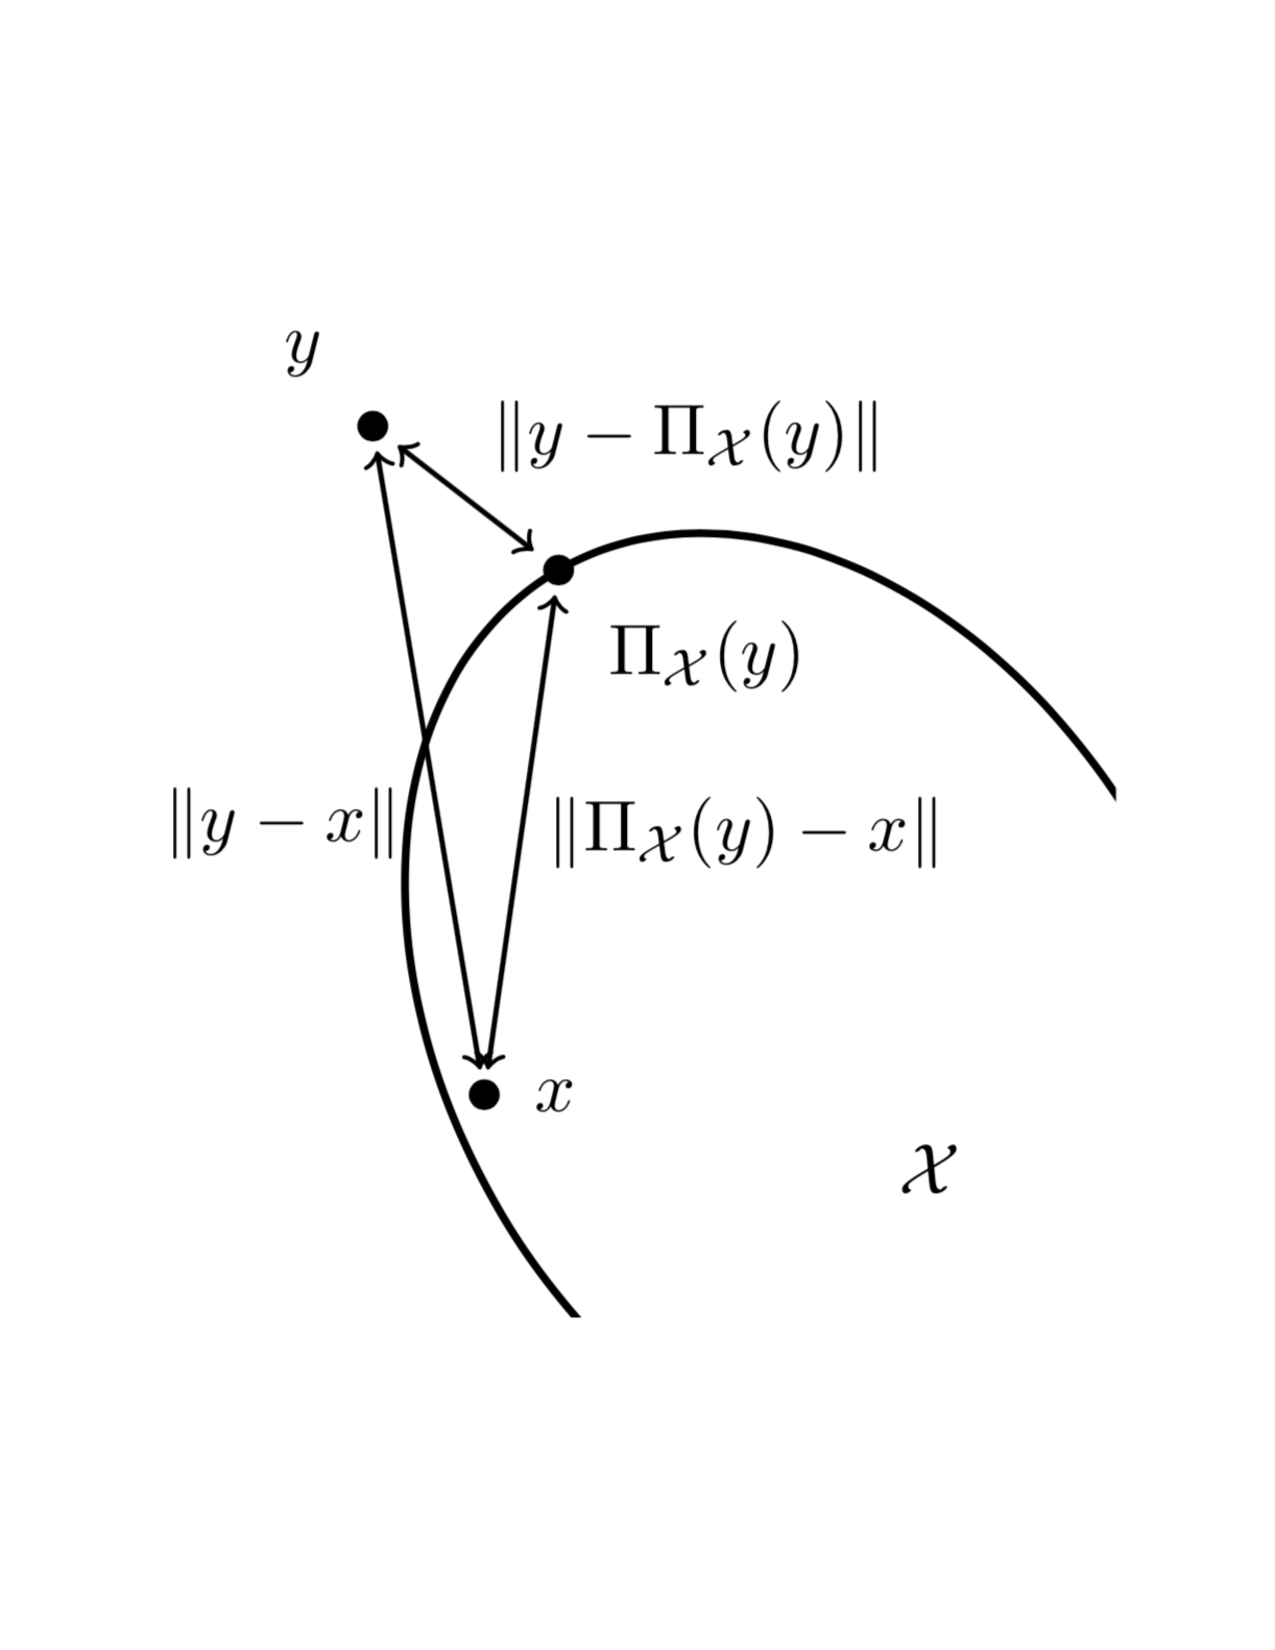
\includegraphics[width=3in]{figures/lecture2-projection}
\end{center}
\caption{Projection of $y$ onto set $\mathcal{X}$. (Figure taken from Bubeck) }
\figurelabel{project}
\end{figure}

The crucial property of projections is that they satisfy the following condition:
\[
\| \Pi_{\domain}(y) - x \|^2 \leq \| y - x \|^2
\]
i.e. the projection of $y$ onto a convex set containing $x$ is closer to $x$. See \figureref{project} for a geometric picture.

\begin{lemma}\lemmalabel{pythagorean}
\[
\| \Pi_{\domain}(y) - x \|^2 \leq \| y - x \|^2 - \| y - \Pi_{\domain}(y) \|^2
\]
Which follows from the Pythagorean theorem. Note that this lemma implies the above property.
\end{lemma}

\subsubsection{Modifying Gradient Descent with Projections}

So now we can modify our original procedure to use two steps.
\[
y_{t+1} = x_t - \eta \nabla f(x_t)
\]
\[
x_{t+1} = \Pi_{\domain}(y_{t+1})
\]

And we are guaranteed that $x_{t+1}\in\domain$. Note that computing the
projection may be the hardest part of your problem, as you are computing an
$\argmin$. However, there are convex sets for which we know explicitly how to
compute the projection (see \exampleref{euclidean-ball}).

\subsection{Convergence Rate of Gradient Descent for $L$-Lipschitz Functions}

\begin{theorem}[Projected Gradient Descent for $L$-Lipschitz Functions]
\theoremlabel{lipschitz}

Assume that function $f$ is convex, differentiable, and closed with bounded
gradients. Let $L$ be the Lipchitz constant of $f$ over the convex domain
$\Omega$. Let $R$ be the upper bound on the distance $\lVert x_1 - x^* \rVert_2$
from the initial point $x_1$ to the optimal point $x^* = \arg\min_{x \in \Omega} f(x)$.
Let $t$ be the number of iterations of project gradient descent.
If the learning rate $\eta$ is set to $\eta=\frac{R}{L \sqrt(t)}$,
then $$f\left(\frac{1}{t}\sum_{s=1}^t x_s\right) - f\left(x^*\right) \leq
\frac{RL}{\sqrt{t}}.$$
\end{theorem}

This means that the difference between the functional value of the average
point during the optimization process from the optimal value is bounded above
by a constant proportional to $\frac{1}{\sqrt{t}}$.

Before proving the theorem, recall the "Fundamental Theorem of Optimization",
which is that an inner product can be written as a sum of norms: $u^\trans v =
\frac{1}{2}(\lVert u \rVert^2 + \lVert v \lVert^2 - \lVert u - v \rVert^2$.
This property can be seen by writing $\lVert u - v \rVert$ as $\lVert u - v
\rVert = \lVert u \rVert^2 + \lVert v \lVert^2 - 2 u^\trans v$.

\begin{proof}[Proof of \theoremref{lipschitz} for compact sets.]

The proof begins by first bounding the difference in function values $f(x_s) -
f(x^*)$.

\begin{align}
    f(x_s) - f(x^*) &\leq \nabla f(x_s)^\trans (x_s - s^*) \equationlabel{a} \\
    &= \frac{1}{\eta}(x_s - y_{s+1})^\trans(x_s - x^*) \equationlabel{b} \\
    &= \frac{1}{2\eta} \left(\lVert x_s - x^* \rVert^2 + \lVert x_s - y_{s+1} \rVert^2 - \lVert y_{s+1} - x^* \rVert^2 \right) \equationlabel{c} \\
    &= \frac{1}{2\eta} \left(\lVert x_s - x^* \rVert^2 - \lVert y_{s+1} - x^* \rVert^2 \right) + \frac{\eta}{2} \lVert \nabla f(x_s) \rVert^2 \equationlabel{d} \\
    &\leq \frac{1}{2\eta} \left(\lVert x_s - x^* \rVert^2 - \lVert y_{s+1} - x^* \rVert^2 \right) + \frac{\eta L^2}{2} \equationlabel{e} \\
    &\leq \frac{1}{2\eta} \left(\lVert x_s - x^* \rVert^2 - \lVert x_{s+1} - x^* \rVert^2 \right) + \frac{\eta L^2}{2} \equationlabel{f}
\end{align}

\equationref{a} comes from the definition of convexity. \equationref{b} comes
from the update rule for projected gradient descent. \equationref{c} comes from
the ``Fundamental Theorem of Optimization.'' \equationref{d} comes from the
update rule for projected gradient descent. \equationref{e} is because $f$ is
$L$-Lipchitz. \equationref{f}
comes from \lemmaref{pythagorean}.

Now, sum these differences from $s=1$ to $s=T$:

\begin{align}
   \sum_{s=1}^t f(x_s) - f(x^*) &\leq  \frac{1}{2\eta} \sum_{s=1}^t \left(\lVert x_s - x^* \rVert^2 - \lVert x_{s+1} - x^* \rVert^2 \right) + \frac{\eta L^2 t}{2} \equationlabel{g} \\
   &= \frac{1}{2\eta} \left(\lVert x_1 - x^* \rVert^2 - \lVert x_{t} - x^{*} \rVert^2 \right) + \frac{\eta L^2 t}{2} \equationlabel{h} \\
   &\leq \frac{1}{2\eta} \lVert x_1 - x^* \rVert^2 + \frac{\eta L^2 t}{2} \equationlabel{i} \\
   &\leq \frac{R^2}{2\eta} + \frac{\eta L^2 t}{2} \equationlabel{j}
\end{align}

\equationref{h} is because \equationref{g} is a telescoping sum.
\equationref{i} is because $\lVert x_{t} - x^* \rVert^2 \geq 0$.
\equationref{j} is by the assumption that $\lVert x_1 - x^* \rVert^2 \leq R^2$.

Then bound $f\left(\frac{1}{t}\sum_{s=1}^t x_s\right) - f\left(x^*\right)$ by
the above sum:

\begin{align}
    f\left(\frac{1}{t}\sum_{s=1}^t x_s\right) &\leq \frac{1}{t} \sum_{s=1}^t f(x_s) \equationlabel{k} \\
    \left(\frac{1}{t}\sum_{s=1}^t x_s\right) - f\left(x^*\right) &\leq \frac{1}{t} \sum_{s=1}^t f(x_s) - f\left(x^*\right) \equationlabel{l} \\
    &\leq \frac{R^2}{2\eta} + \frac{\eta L^2 t}{2}
\end{align}

\equationref{k} is by convexity. $\frac{R^2}{2\eta} + \frac{\eta L^2 t}{2}$,
the upper bound of the difference between $f\left(\frac{1}{t}\sum_{s=1}^t
x_s\right)$ and $f\left(x^*\right)$ is minimized when $\eta$ is set to be
$\frac{RL}{\sqrt{t}}$.

\end{proof}

\subsection{Convergence Rate of Gradient Descent for $\beta$-Smooth Functions}

\begin{definition}[$\beta$-smoothness]
A continuously differentiable function f is $\beta$ smooth if the gradient $\nabla f$ is $\beta$-Lipschitz, i.e
$$||\nabla f(x) - \nabla f(y)|| \leq \beta||x-y||$$
\end{definition}

We will show that gradient descent with the update rule
$$x_{t+1} = x_t - \eta \nabla f(x_t)$$
attains a faster rate of convergence under the smoothness condition.

\begin{theorem}
Let $f$ be convex and $\beta$-smooth on $\R^n$ then gradient descent with $\eta = \frac{1}{\beta}$ satsifies
$$f(x_t) - f(x^*) \leq \frac{2\beta||x_1 - x^*||^2}{t-1}$$
\end{theorem}
To prove this we will need the following two lemmas.

\begin{lemma}\label{l1}
Let $f$ be a $\beta$-smooth function on $\R^n$.  Then for any $x,y \in \R^n$, one has
$$|f(x) - f(y) - \nabla f(y)^T(x-y)| \leq \frac{\beta}{2}||x-y||^2$$
\end{lemma}

\begin{proof}
First represent $f(x) - f(y)$ as an integral, apply Cauchy-Schwarz and then $\beta$-smoothness:

$$|f(x) - f(y) - \nabla f(y)^T(x-y)|$$
$$= \big|\int\limits_{0}^1 \nabla f(y + t(x-y))^T(x-y)dt - \nabla f(y)^T(x-y)\big|$$
$$\leq  \int\limits_{0}^1 ||\nabla f(y + t(x-y)) - \nabla f(y)||\cdot ||x-y||dt$$
$$\leq \int\limits_{0}^1 \beta t||x-y||^2dt$$
$$= \frac{\beta}{2}||x-y||^2$$
\end{proof}

We also need

\begin{lemma} \label{lm2}
Let $f$ be a $\beta$-smooth function, then for any $x,y \in \R^n$, one has
$$f(x) - f(y)\leq \nabla f(x)^T(x-y) - \frac{1}{2\beta}||\nabla f(x) - \nabla f(y)||$$
\end{lemma}

\begin{proof}
Let $z = y - \frac{1}{\beta}(\nabla f(y) - \nabla f(x))$.  Then one has

$$f(x) - f(y)$$
\begin{align}
    &= f(x) - f(z) + f(z) - f(y) \\
    &\leq \nabla f(x)^T(x-z) + \nabla f(y)^T(z-y) + \frac{\beta}{2}||z-y||^2 \\
    &= \nabla f(x)^T(x-y) + (\nabla f(x) - \nabla f(y))^T(y-z) + \frac{1}{2\beta}||\nabla f(x) - \nabla f(y)||^2 \\
    &= \nabla f(x)^T(x-y) - \frac{1}{2\beta} ||\nabla f(x) - \nabla f(y)||^2
\end{align}

\end{proof}

Now we prove the theorem

\begin{proof}
By the update rule and lemma \ref{l1} we have
$$f(x_{s+1}) - f(x_s) \leq -\frac{1}{2\beta}||\nabla f(x_s)||^2 $$
In particular, denoting $\delta_s = f(x_s) - f(x^*)$ this shows
$$\delta_{s+1} \leq \delta_s - \frac{1}{2\beta}||\nabla f(x_s)||^2 $$
One also has by convexity
$$\delta_s \leq \nabla f(x)s)^T(x_s - x^*) \leq ||x_s - x^*|| \cdot ||\nabla f(x_s)||$$
We will prove that $||x_s - x^*||$ is decreasing with $s$, which with the two above displays will imply
$$\delta_{s+1}\leq \delta_s - \frac{1}{2\beta||x_1 - x^*||^2}\delta_s^2$$
We solve the recurrence as follows.  Let $w = \frac{1}{2\beta||x_1 - x^*||^2}$, then
$$w\delta_s^2 + \delta_{s+1} \leq \delta_s \iff w\frac{\delta_s}{\delta_{s+1}} + \frac
{1}{\delta_s} \leq \frac{1}{\delta_{s+1}} \implies \frac{1}{\delta_{s+1}} - \frac{1}{\delta_s} \geq w \implies \frac{1}{\delta_t} \geq w(t-1)$$
To finish the proof it remains to show that $||x_s - x^*||$ is decreasing with $s$.  Using lemma \ref{lm2} one immediately gets
$$ (\nabla f(x) - \nabla f(y))^T(x - y) \geq \frac{1}{\beta} ||\nabla f(x) - \nabla f(y)||^2$$
We use this and the fact that $\nabla f(x^*) = 0$
\begin{align}
    ||x_{s+1} - x^*||^2 &= ||x_s - \frac{1}{\beta}\nabla f(x_s) - x^*||^2 \\
    &= ||x_s - x^*||^2 - \frac{2}{\beta}\nabla f(x_s)^T(x_s - x^*) + \frac{1}{\beta^2}||\nabla f(x_s)||^2 \\
    &\leq ||x_s - x^*||^2 - \frac{1}{\beta^2} ||\nabla f(x_s)||^2 \\
    &\leq ||x_s - x^*||^2
\end{align}
which concludes the proof.
\end{proof}

